\section{Discussion and Future Work}
\label{sec:disc}

\noindent \textbf{Multithreaded CPU Processing.} The comparison of our CPU/GPU
router to the CPU-only baseline is not completely fair. Our CPU-only router
operates in a single thread, yielding misleadingly low performance. Any
CPU-based software router in the real world would certainly spread packet
processing across multiple cores, and we would be surprised if any core
software router were run on a machine with fewer than 16 cores.

A simple extension of our project would be to parallelize our CPU-only packet
processing functions with OpenMP to provide more realistic baseline
measurements.

We have implemented a simple multi-threaded version. Our preliminary results show that OpenMP can dramatically improve the performance. By tuning the number of threads and the batch size, we could increase the bandwidth up to one order of magnitude, with respect to the mono-thread version. However, the packet processing on the GPU still outperforms that on the CPU, being around 20\% faster. More investigation is however required to understand the impact of the parameters on the performance.

\medskip \noindent \textbf{Harder Processing Functions.} Even in the final
iteration of our router, the CPU/GPU version only achieves slightly more than
three times the bandwidth of the CPU-only version. Though this is by no means
an improvement to scoff at, the speedup strikes us as being a tad low. We
suspect the cause is that our packet processing functions are not taxing
enough; the harder the processing function, the more benefit we should see from
the massively parallel GPU. This suggests that GPU-based software routers might
be best suited for complex packet processing like IDS filtering (which requires
pattern matching against packet payloads) and IPsec processing (which requires
expensive cryptographic operations).

One of our goals was to explore the best way to schedule multiple packet
processing functions on the GPU. As a simple example, to schedule both LPM and
firewall lookup, you could imagine parallelizing per-packet or parallelizing
per-function (Figure~\ref{fig:scheduling}). We began testing these schemes,
but, as our processing functions turned out to be ``easy,'' there was little
difference. We think this is still an interesting question to explore with more
taxing processing functions.

\begin{figure}
    \centering
    \subfigure[Per-packet]{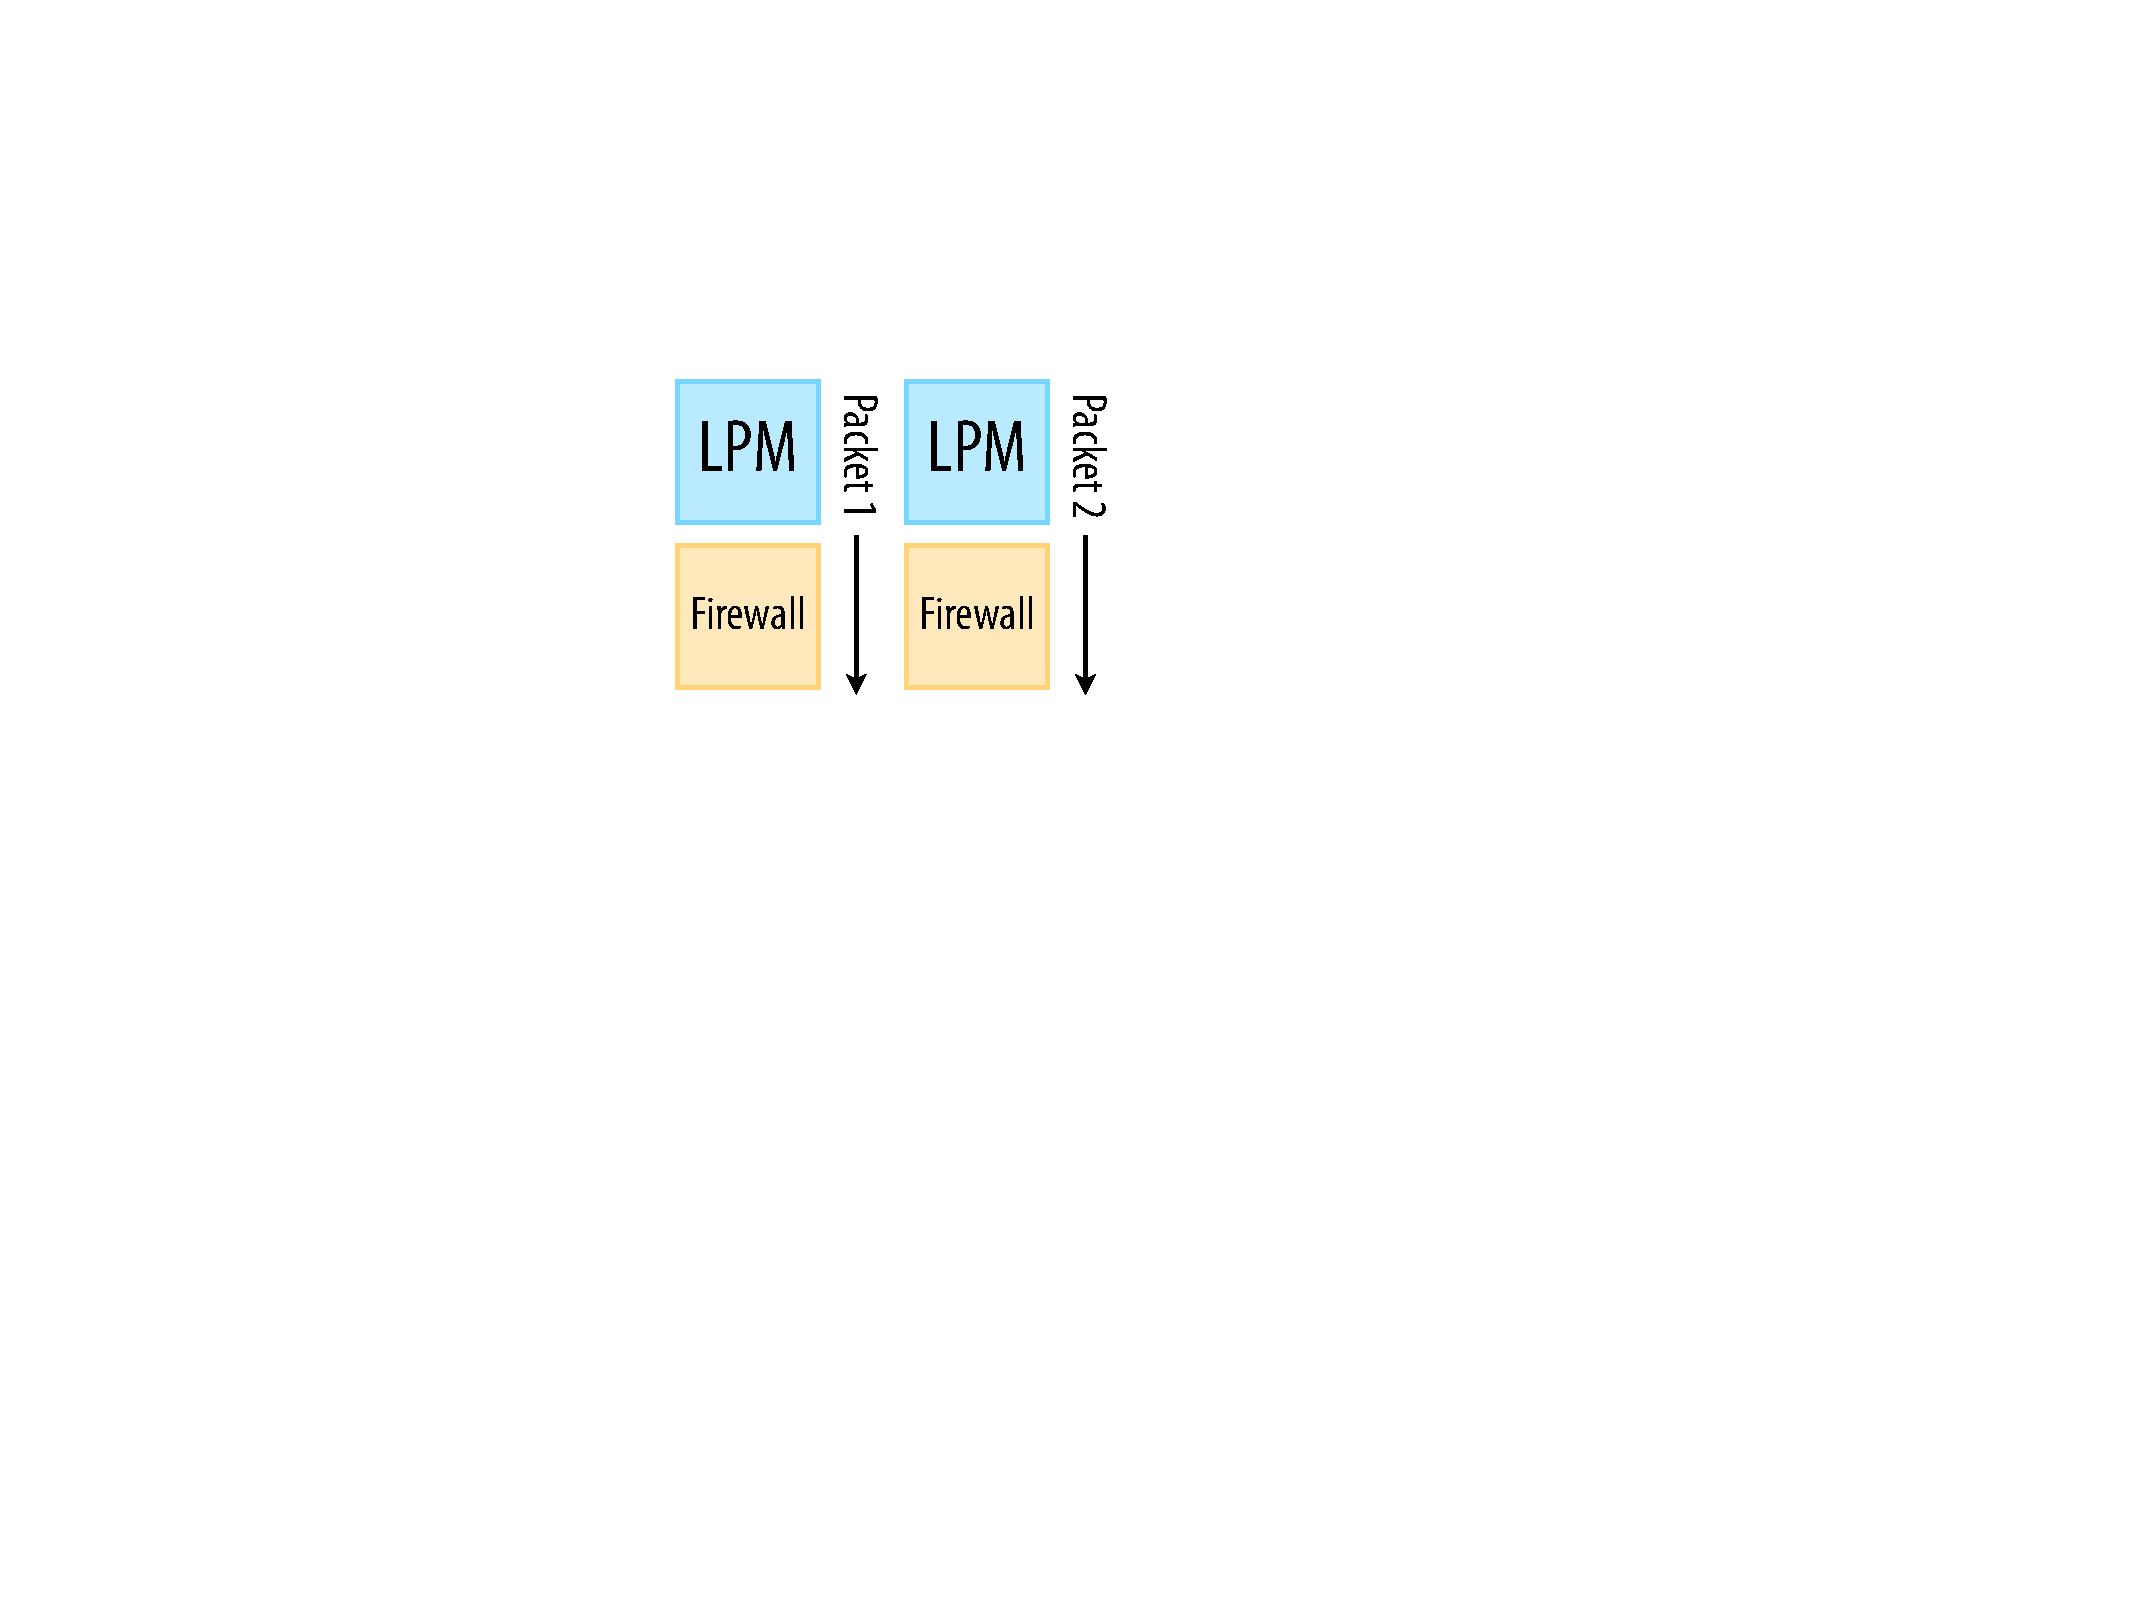
\includegraphics[height=3cm]{figs/per-packet-par.pdf}\label{fig:per-packet-par}}

	\medskip
    \subfigure[Per-function per-packet]{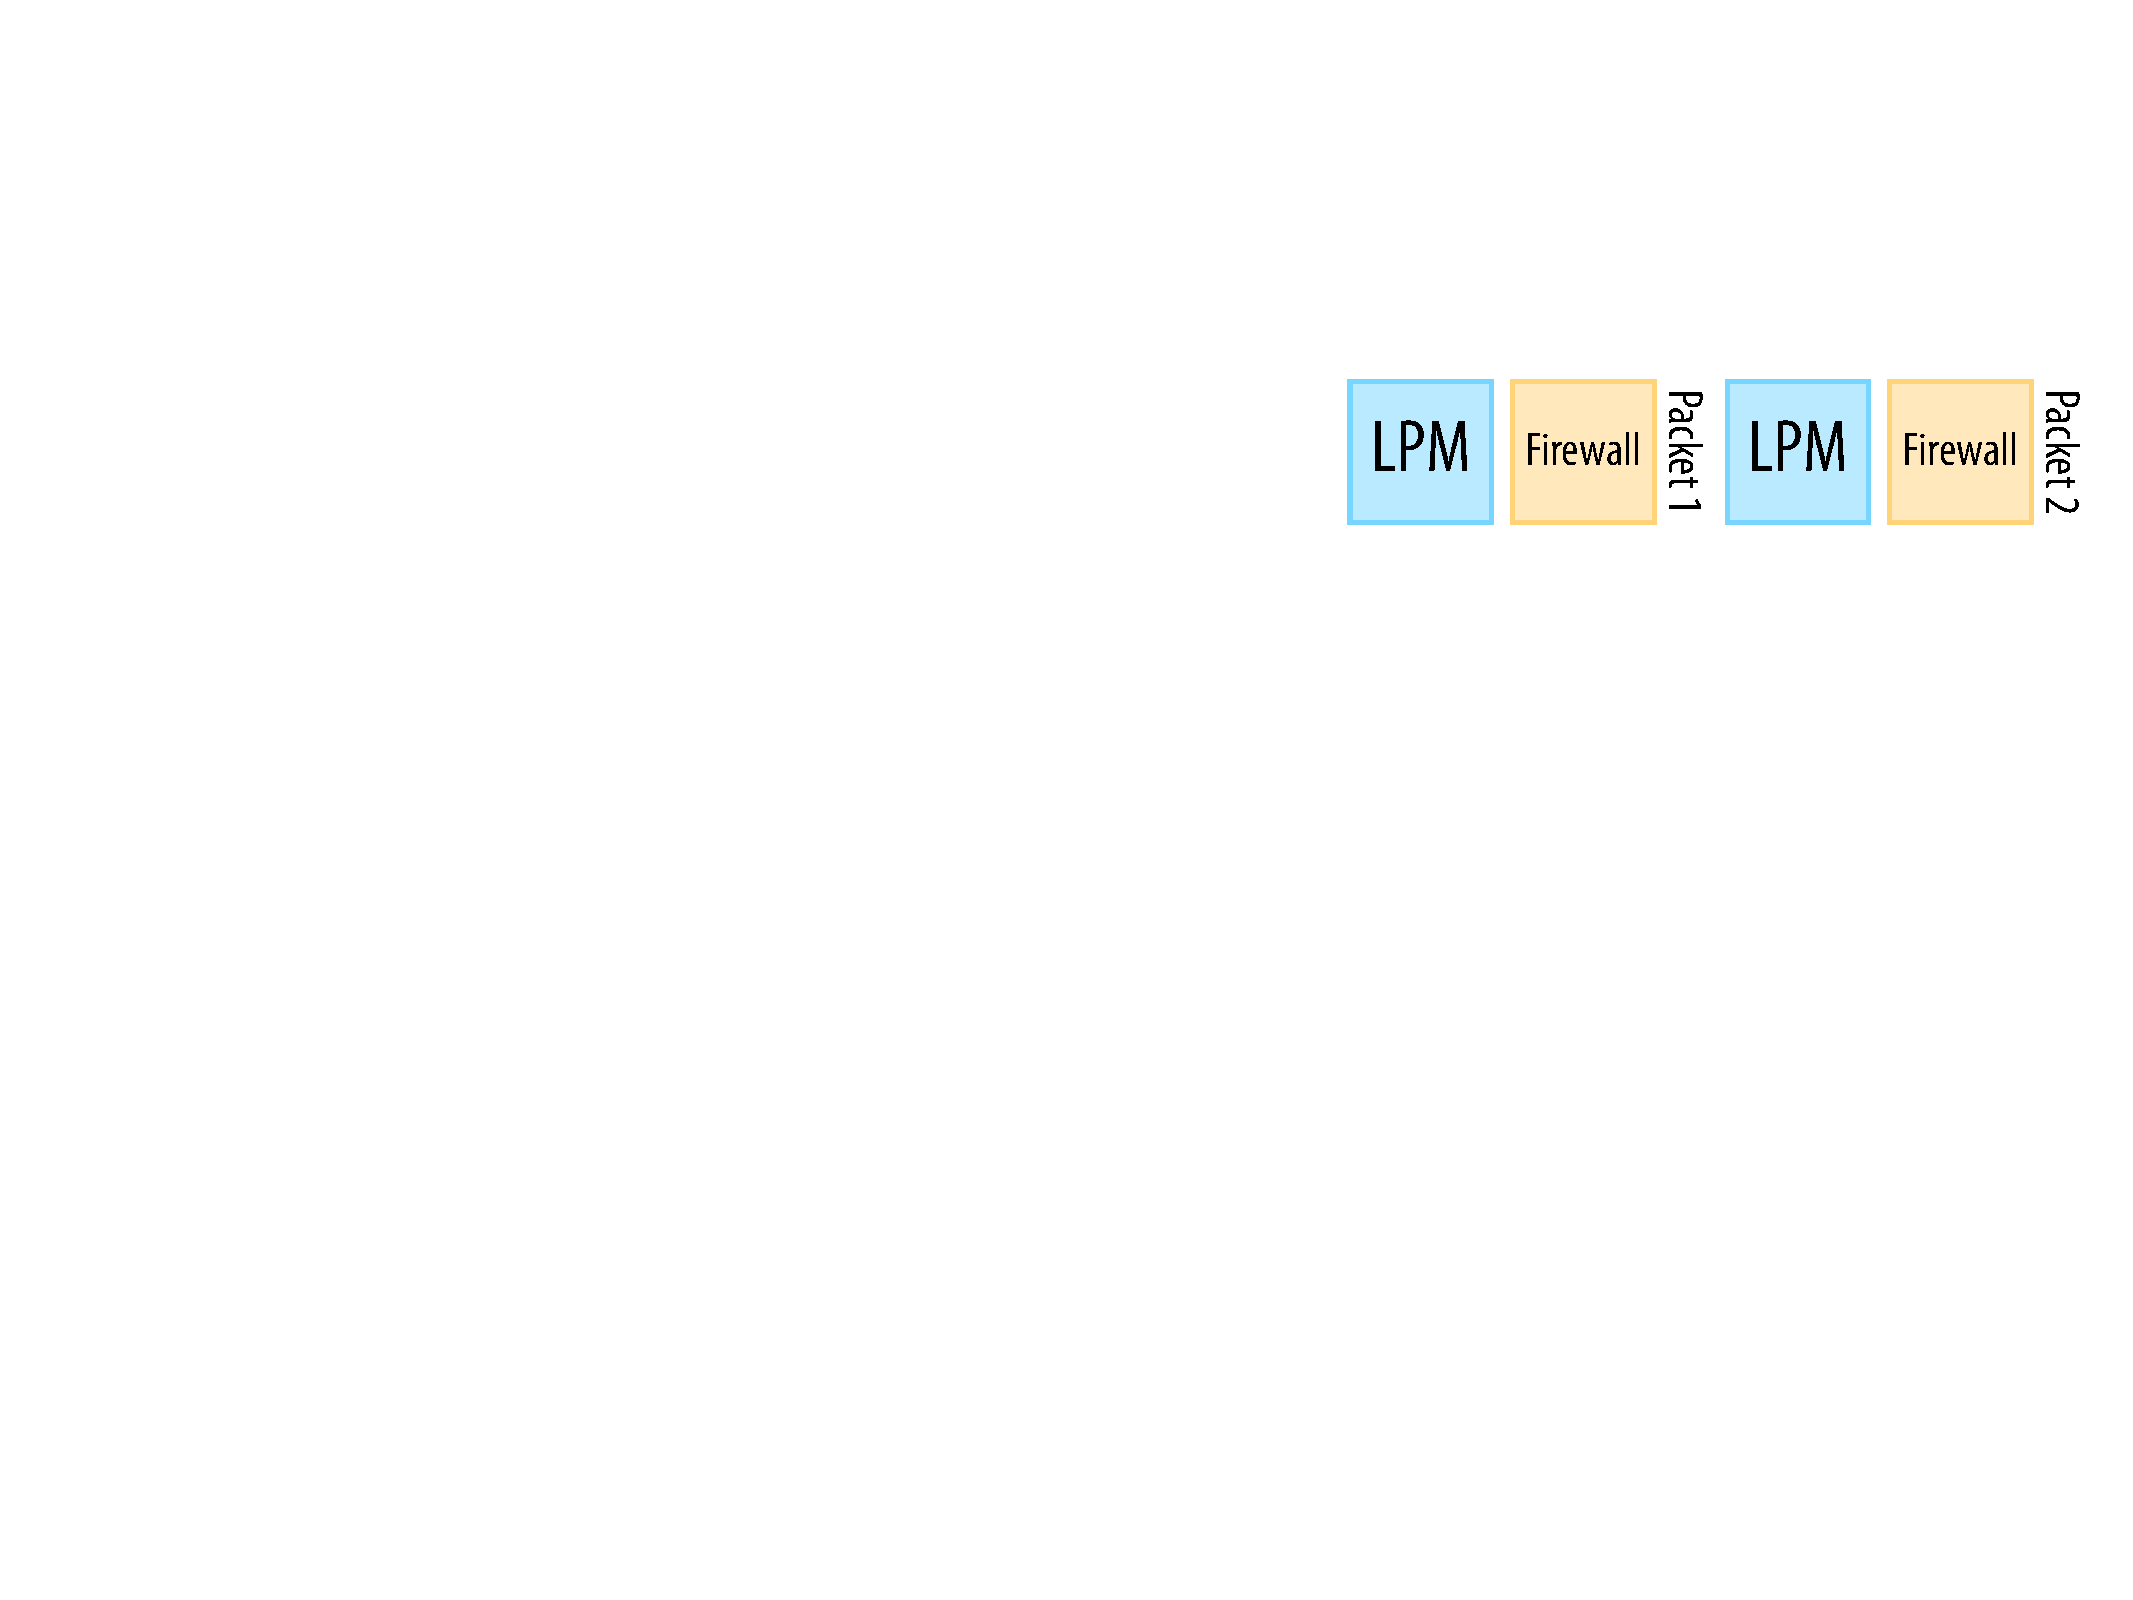
\includegraphics[height=1.5cm]{figs/per-function-par.pdf}\label{fig:per-function-par}}

    \caption{Scheduling Multiple Processing Functions}
	\label{fig:scheduling}
\end{figure}

\medskip \noindent \textbf{Faster Packet I/O.} By far the largest issue we noted
is that generating and gathering packets from Click contributes to the majority
of the latency, becoming the dominant part of both CPU and GPU overall
latency. As seen in Figure \ref{fig:iter4}, removing the overhead contributed by
generating and gather packets, our GPU implementation performs much better than
our CPU implementation. This is the same conclusion that the authors of
PacketShader \cite{Han} came to. Thus in their system, they focused on
reimplementing the driver for their NIC to alleviate these issues. In our
framework we could similarly emulate newer NIC technologies (like RDAM) to allow
zero-copy access to DRAM that is memory mapped in the GPU. We could emulate this
by having Click copy packets directly to application DRAM rather than first
sending the packets to the application via a socket.

\medskip \noindent \textbf{Streams.} The typical use of a GPU involves the
following operations: a set of tasks and input data is first collected,
transferred to the GPU, processed, and eventually the output is copied back to
the host device. These operations are performed cyclically, often on
independent data, as in the case of our packet processing applications. Since
the CUDA and host device are separate processing unit, it is critical for
performance to maximize the concurrency of such operations.

CUDA Streams provide an interesting mechanism to optimize GPU-based
applications. Basically, CUDA allows to assign operations (like kernel
execution and \emph{asynchronous} data transfer to and from the device) to
streams. Then, the stream executions are overlapped in such a way that similar
operations of different streams do not interfere with each other (i.e., a kernel
execution in stream1 and a data transfer in stream2 can be performed in
parallel). The high level idea is quite similar to that of instruction
pipelining.

We have implemented a version of our router using CUDA streams. Our preliminary
results show that streams indeed increase the parallelism and throughput.
Operation overlapping is quite visible in the Visual Profiler. The number of
processed packets increases substantially (around 30-40\%). However, more
investigation is required on this subject, particularly on the packet generator
and on the new issues related to resource management, highlighted by the Visual
Profiler.

%\TODO{Bruno: Briefly describe CUDA's built-in streams funcitonality}

\medskip \noindent \textbf{Integrated Graphics Processors.} One tempting idea
to explore is the use of integrated graphics processors rather than dedicated
discrete GPUs. Modern processors (Intel Core i-series, etc.) include a
traditional multi-core GPU directly on the processor itself. In essence, this
shifts the position of the GPU from being on the PCI-express bus to being
co-located with the CPU on the quickpath interconnect (QPI). As the QPI can
potentially provide more bus bandwidth to memory, and integrated graphics
processor could obtain even higher maximum throughput, as memory constraints
are the biggest source of potential slowdown after packet I/O at the NIC.
